\documentclass[a4paper,12pt]{report}

\usepackage{alltt, fancyvrb, url}
\usepackage{graphicx}
\usepackage[utf8]{inputenc}
\usepackage{float}
\usepackage{hyperref}

% Questo commentalo se vuoi scrivere in inglese.
% \usepackage[italian]{babel}

% \usepackage[italian]{cleveref}
\usepackage{cleveref}

\title{Homer}

\author{Ceccacci Michele, Magnani Simone, Monticelli Alessandro}
\date{\today}


\begin{document}

\maketitle

\begin{abstract}
\end{abstract}

\tableofcontents

\chapter{Analysis}
\section{Requirements}

HOMER (HOMe EmulatoR) is an emulated domotic controller connected to lights, windows, and other domestic facilities.
The smart environment is managed through a dashboard which allows the user to control devices, monitor sensors and electrical consumptions.
Each device should support updates in variable time units.
Some devices should act in a somewhat random way (but still predictable), while others should be fully deterministic.

\subsubsection{Functional Requirements}

\begin{itemize}
	\item The software should allow creating and controlling lots of different devices, such as:
	\begin{itemize}
		\item Lights
		\item Electrical outlets
		\item Doors
		\item Locks
		\item Windows
		\item Blinds
		\item Temperature changer devices
	\end{itemize}
	\item Devices can be added/removed at runtime.
	\item A logger is needed in order to allow users to keep track of state changes. It also makes debugging easier for developers.
	\item The software should have graph views for temperature and air quality state.
	\item The users should be able to see electrical consumption.
	\item The users should be able to set the desired temperature in the course of the day.
	\item The users should be able to view the trend of temperature, consumptions and air quality.
\end{itemize}

\subsubsection{Non-Functional Requirements}

\begin{itemize}
	\item Should be performant enough to run on a desktop/laptop.
	\item User interface should be intuitive and user-friendly
	\item The project should be portable, and work on Windows, MacOS and Linux devices.
\end{itemize}

\section{Analysis and domain model}
\subsection[]{Domain analysis}

The application will emulate a domotic environment, some smart devices and facilities monitoring.
Smart devices are common domestic devices as lights, electrical outlets, windows, doors and various sensors 
for monitoring indoor temperature and air quality along with electrical absorption.
The user will interact with the devices via the controller through a dashboard.

The main challenge will be modelling the communication between the controller 
and the different devices, which can have very different states.

\begin{figure}[H]
\centering{}
\includegraphics[width=\textwidth,height=\textheight,keepaspectratio]{uml/domain.png}
\caption{UML diagram of the domain}
\label{uml:domain}
\end{figure}

\chapter{Design}
\section{Architecture}

HOMER is built on the MVC (model-view-controller) architecture. 
The controller is responsible for getting inputs from the views, and updating the model consequently.
The controller also sends back state updates to the various views.
The model part is composed by the devices and electrical outlets. Each device has a state of its own, that
the controller gets and sends to the views. 
Each view is independent from each other, and when a view commands a state update
the controller processses the change and then updates all the views.

\begin{figure}[H]
\centering{}
\includegraphics[width=\textwidth,height=\textheight,keepaspectratio]{uml/architecture.png}
\caption{UML diagram of the architecture}
\label{uml:architecture}
\end{figure}

\section{Detailed Design}
Problem: Sending updates from the view to the controller. 
We need a common way for all the UI components to send the same kind of updates to the controller without repeating code.
We also want the controller to have more control over what is actually execute, and when it is executed. So the controller acts as a receiver.
All the commands implement an execute method, that is called inside the controller.
Solution: Used the command pattern, which allows %TODO needs better phrasing and a uml diagram 
different views to send the same updates to the controller, avoiding code duplication
Commands that create devices need to be displayed to the user, so we created a new interface called CreateDeviceCommand
and we decided to opt for string representations instead of enums to allow for further expansibility.
\newline
\includegraphics[width=12cm]{uml/command.png}



\subsection{Michele Ceccacci}

\subsubsection{Logger} 
Problem: The system needs a composable logger, which has to track both state updates in devices and connections/disconnections
of devices. The need for composition stems from the fact that different use cases of the software might need just a subset
of the logging capabilities. The logger must also be dynamically composable for maximum flexibility.
Solution: used the Decorator design pattern, which allows to wrap dynamically objects at runtime and compose them.
Not using abstract classes also takes away the problems of inheritance. \newline
\includegraphics[width=16cm]{uml/logger.png}

\subsubsection{Air conditioning and Heating}
Problem: 
Air conditioning and Heating devices have really similar behaviours. The difference between the two, is that an air conditioning
device decreases the environment's temperature, whereas the heating device raises it.
Solution: Since the only function that actually changes between the two implementations is the one responsible for updating the
environment's temperature, the template method pattern was used. 
The method updateTick, responsible to update the environment and electrical consumption when called by the controller,
is a template method, and calls the abstract method updateTemperature. \newline

\includegraphics[width=16cm]{uml/abstractTemperaturechanger.png}

\subsubsection{Passing state updates to the view}
Problem: devices have really different states, and they all need to passed down to the view.
I took inspiration from REST applications, and implemented a DeviceState interface, which all device states would implement.
Then i defined a single command for state updates, so that the view could create a component for the specific device in case
the device wasn't already present. For device removals, i just created a single removeDevice Method in the DeviceViewer interface, 
based on the deviceId. \newline % TODO this could be far better.

\subsection{Simone Magnani}

\subsubsection{Simulation}

The simulation is a \texttt{discrete-time simulation}, where each tick represents an amount of time that has passed.
This allows to control the \texttt{delta time}, therefore allowing to speed up/down the simulation.

Any component that requires to update its state in steps and know how much time
has passed will implement the interface \texttt{DiscreteObject}.

\begin{figure}[H]
\centering{}
% 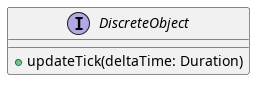
\includegraphics[width=\textwidth,height=\textheight,keepaspectratio]{magnani/uml/discreteobject.png}
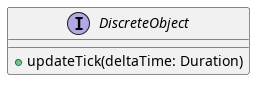
\includegraphics[keepaspectratio]{magnani/uml/discreteobject.png}
\caption{UML diagram of the DiscreteObject interface}
\label{magnani:uml:discreteobject}
\end{figure}

\paragraph{Problem} Since the simulation can be sped up, we have to track the time in the simulation environment
\paragraph{Solution} Creation of the concept of \texttt{Clock} that stores the time and is updated at each tick.

\begin{figure}[H]
\centering{}
% 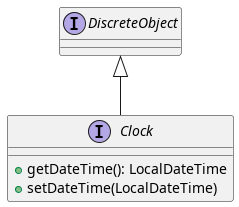
\includegraphics[width=\textwidth,height=\textheight,keepaspectratio]{magnani/uml/clock.png}
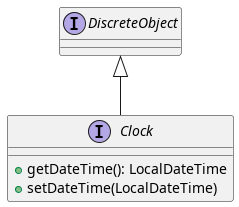
\includegraphics[keepaspectratio]{magnani/uml/clock.png}
\caption{UML diagram of the clock}
\label{magnani:uml:clock}
\end{figure}

\subsubsection{Control of the simulation}

The game loop is handled in the simulation manager.

The simulation manager logic is split between the \texttt{SimManager} and \texttt{SimManagerViewObserver}.

Any \texttt{DiscreteObject} can ask to be updated by the game loop with the
\texttt{Observer} pattern,via the \texttt{SimManager} method \texttt{addObserver}.

The simulation manager interfaces with its view counterpart to allow pause/resume
and time rate control via the \texttt{SimManagerViewObserver} using the \texttt{Observer} pattern.

\begin{figure}[H]
\centering{}
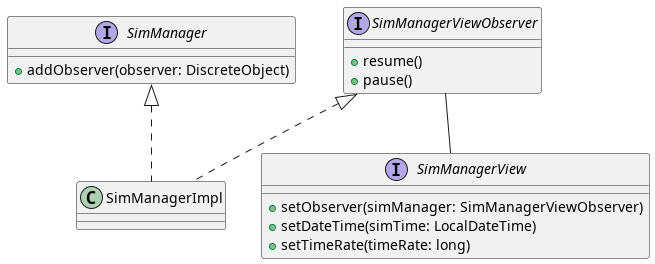
\includegraphics[width=\textwidth,height=\textheight,keepaspectratio]{magnani/uml/simmanager.png}
\caption{UML diagram of the SimulationManager}
\label{magnani:uml:simmanager}
\end{figure}

\subsubsection{Devices}

Devices will be detailed separarely between read-only, toggleable and adjustable ones.

\subsubsection{Thermometer}

The thermometer is modelled as an extension of \texttt{Device} since it's not meant to be controllable
but only to return a \texttt{DeviceState} to the Controller,
and \texttt{DiscreteObject}, to define how should the temperature be sensed (in
a simple case, it could be updated directly, or in another case imperfections such as lag can be modelled).

% The DiscreteObject could also have been directly implemented instead of being extended by Thermometer,
% but I wanted to put 

\begin{figure}[H]
\centering{}
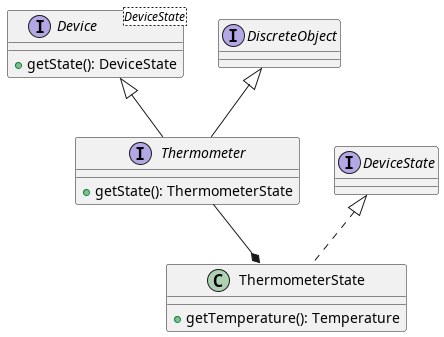
\includegraphics[width=\textwidth,height=\textheight,keepaspectratio]{magnani/uml/thermometer.png}
\caption{UML diagram of the thermometer}
\label{magnani:uml:thermometer}
\end{figure}

\paragraph{Problem} There are multiple devices that need to interact with a common temperature
\paragraph{Solution} Creation of the concept of \texttt{Environment} which represents the
physical simulated environment with its temperature parameter.
In the future, this would also allow to simulate different environments, eg. different rooms or completely
separate buildings.

\begin{figure}[H]
\centering{}
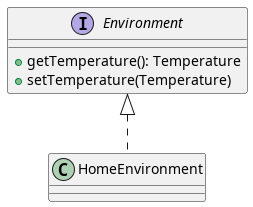
\includegraphics[keepaspectratio]{magnani/uml/environment.png}
\caption{UML diagram of the environment}
\label{magnani:uml:environment}
\end{figure}

\subsubsection{Lock}

The Lock has been modelled as a \texttt{ToggleableDevice}.
Its logic is really simple, the state can vary between locked and unlocked.
The lock is represented in figure \Cref{magnani:uml:lock}

\begin{figure}[H]
\centering{}
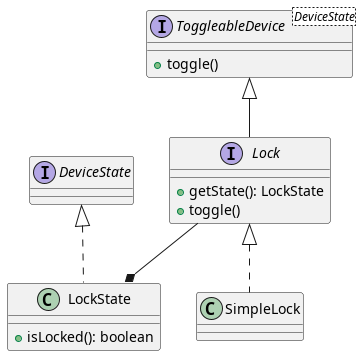
\includegraphics[width=10cm,height=\textheight,keepaspectratio]{magnani/uml/lock.png}
\caption{UML diagram of the lock}
\label{magnani:uml:lock}
\end{figure}

\subsubsection{Window, Door, Blinds}

The devices of type \texttt{Window, Door and Blinds} are modelled as \texttt{AdjustableDevice}s.

\paragraph{Problem} Each of these devices can be considered to be controllable between a range of values. Also, if those devices
were meant to be remotely controllable, there should be something that moves them.
\paragraph{Solution} Create the concept of \texttt{Actuator}. This also allows someone to decide however they want to model
the movement mechanism (as simplistically or realistically as preferred) $=>$ \texttt{Strategy} pattern.
It also allows to compartmentalize away the logic of the movement, adhering to the single responsibility principle.

\paragraph{Problem} Min, max values for ranges (eg. actuator movement range) require to be managed
in several parts. It is also necessary to make sure that the order of the values is correct.
This would lead to a lot of duplicated code.
\paragraph{Solution} Create a \texttt{Bounds} class encapsulating the concept of boundaries,
which also allows to check the correct order of the bounds internally.

\begin{figure}[H]
\centering{}
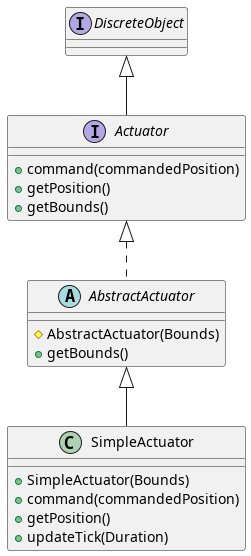
\includegraphics[width=\textwidth,height=12cm,keepaspectratio]{magnani/uml/actuator.png}
\caption{UML diagram of the actuator}
\label{magnani:uml:actuator}
\end{figure}

\paragraph{Problem} Reuse of code for the different devices.
\paragraph{Solution} Create the concept of \texttt{ActuatedDevice}. Then, create an \texttt{AbstractActuatedDevice}
which wraps an \texttt{Actuator}.
It is then possible to create several different implementations and choose which actuator implementation to use,
without having to create other device implementations that would be practically identical.

% Problem: Actuator in MechanizedWindow (we might want to change it eg. use a more realistic one)
% Solution: pass the actuator in the constructor, this allows to use different actuators without having
% to create other Window implementations that would only be different in terms of which actuator is being used.

\begin{figure}[H]
\centering{}
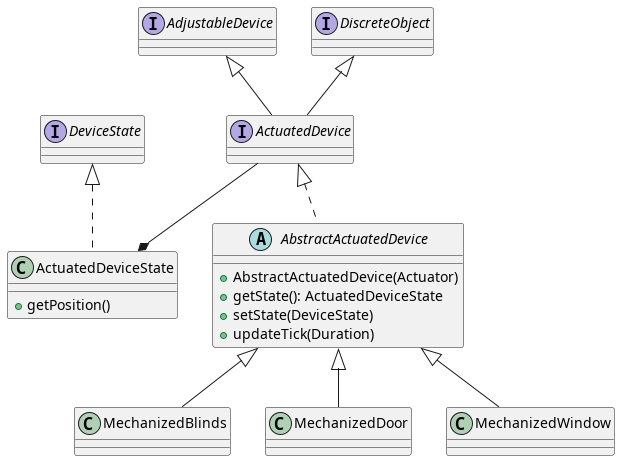
\includegraphics[width=\textwidth,height=\textheight,keepaspectratio]{magnani/uml/actuateddevice.png}
\caption{UML diagram of the ActuatedDevice and how the devices derive from it}
\label{magnani:uml:actuateddevice}
\end{figure}

\subsubsection{Temperature Scheduler}

The temperature scheduler is a component with the task of attaining the user's desired temperature. \newline
It is external of the controller, but interfaces with it in the implementation. \newline
The scheduler has been separated between model, controller and view.
Generics have been used to allow reusability.

\begin{figure}[H]
\centering{}
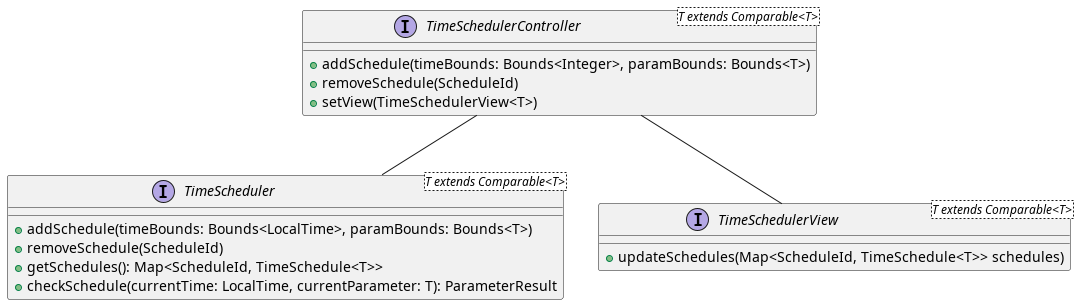
\includegraphics[width=\textwidth,height=\textheight,keepaspectratio]{magnani/uml/scheduler.png}
\caption{UML diagram of the scheduler overall structure}
\label{magnani:uml:scheduler}
\end{figure}

\subsubsection{Scheduler Model}

The scheduler model manages the storage of the schedules and the checking of the current parameter against the schedule.

\begin{figure}[H]
\centering{}
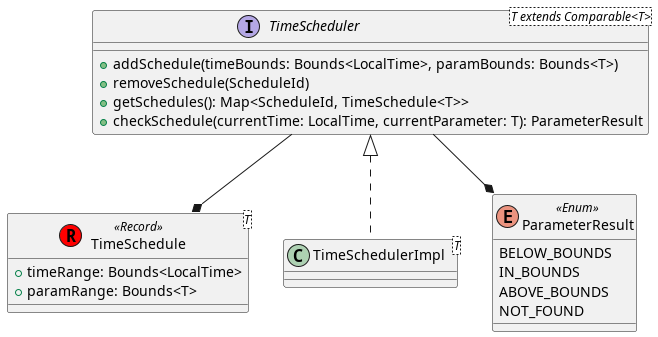
\includegraphics[width=\textwidth,height=\textheight,keepaspectratio]{magnani/uml/scheduler-model.png}
\caption{UML diagram of the scheduler model}
\label{magnani:uml:scheduler-model}
\end{figure}

\subsubsection{Scheduler Controller}

The scheduler controller handles the communication between the model and the view, and also implements the \texttt{DiscreteObject} interface
to periodically ask the model if the target parameter is met.
When the target parameter is not met, the scheduler will send a command to the domotic controller.

\begin{figure}[H]
\centering{}
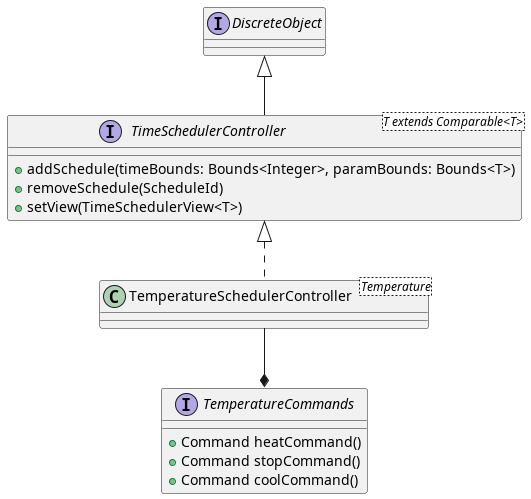
\includegraphics[width=\textwidth,height=\textheight,keepaspectratio]{magnani/uml/scheduler-controller.png}
\caption{UML diagram of the scheduler controller}
\label{magnani:uml:scheduler-controller}
\end{figure}

A \texttt{TemperatureCommands} interface has been created, following the \texttt{Strategy} pattern, to
specifically deal with the control of the temperature. \newline
Three separate commands are expected: heating, cooling, and stopping when the parameters are met.
In the proposed implementation, the heaters and air conditioners are instructed to set their state
to the minimum or maximum possible intensity, but for example, another implementation could
take into account the difference between the current temperature and the desired temperature,
and regulate the intensity proportionally.

A \texttt{Template} pattern has been used in \texttt{TemperatureCommand} to create this implementation,
with an abstract method \texttt{Function} to reuse the same code for both heating and cooling.
The template method is \texttt{setState}, as shown in figure \Cref{magnani:uml:temperaturecommand}.
This method is then used for both the heating and cooling functions.

\begin{figure}[H]
\centering{}
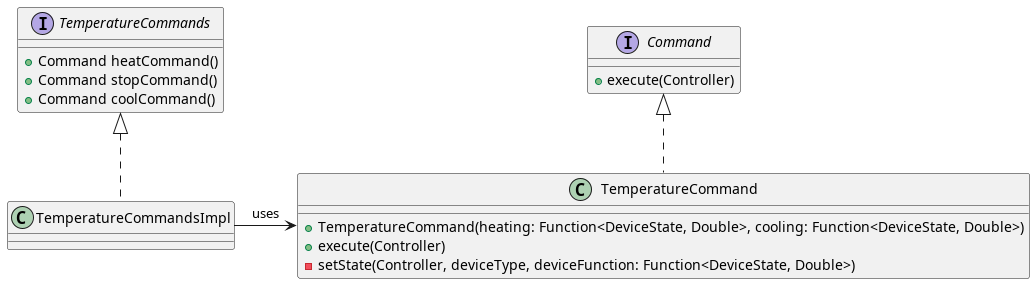
\includegraphics[width=\textwidth,height=\textheight,keepaspectratio]{magnani/uml/temperaturecommand.png}
\caption{UML diagram of the implementation of TemperatureCommands with the use of a template method in TemperatureCommand}
\label{magnani:uml:temperaturecommand}
\end{figure}

\subsubsection{Scheduler View}

The scheduler view has two tasks: allow the user to add/remove schedules, by calling the controller methods,
and displaying the current schedules, when updated from the controller.

\begin{figure}[H]
\centering{}
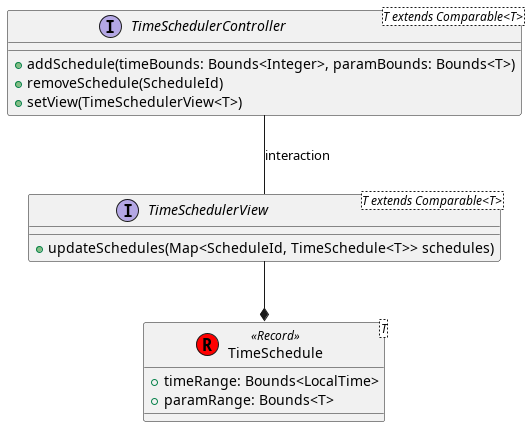
\includegraphics[width=\textwidth,height=\textheight,keepaspectratio]{magnani/uml/scheduler-view.png}
\caption{UML diagram of the scheduler view}
\label{magnani:uml:scheduler-view}
\end{figure}

\subsubsection{Graphs}

As with the scheduler, the implementation of the graphs has been divided between model, controller, and view components.

\subsubsection{Graphs Model}

The model has the simple task of storing the logged data, and providing the dataset upon request.

\begin{figure}[H]
\centering{}
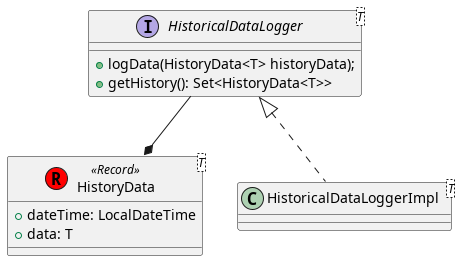
\includegraphics[width=\textwidth,height=\textheight,keepaspectratio]{magnani/uml/graph-model.png}
\caption{UML diagram of the graph model}
\label{magnani:uml:graph-model}
\end{figure}

\subsubsection{Graphs Controller}

The controller has the task of supplying the data to log to the model, and to refresh the view.
It has been generalized with the use of a \texttt{Supplier} in an abstract implementation \texttt{AbstractLogger}. \newline
The supplier decides how to retrieve the data to log, effectively becoming an abstract method, and the updateTick (where the data is logged)
becomes a template method.

\begin{figure}[H]
\centering{}
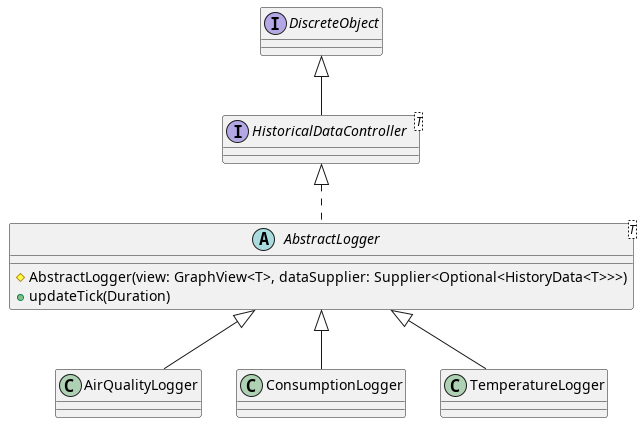
\includegraphics[width=\textwidth,height=\textheight,keepaspectratio]{magnani/uml/graph-controller.png}
\caption{UML diagram of the graph controller}
\label{magnani:uml:graph-controller}
\end{figure}

\paragraph{Problem} We have to choose which thermometer to log.
\paragraph{Solution} Use the first/any thermometer found.
This solution would not work with multiple thermometers in different environments.
In that case it would be better to choose a particular thermometer to log, and/or to have multiple logs for all the different thermometers.

\paragraph{Problem} We have to choose how to log the data.
\paragraph{Solution} I chose to log the data at each (simulation) hour for design simplicity.
Could also have logged each tick, but it would have led to some pretty confusing graphs if the time rate were to be modified
due to the time axis not being linear.
In the future, the time between each log could be configured.
It could also be possible to log more frequently but choose to display at a larger interval of time.

\subsubsection{Graphs View}

The graph view has the task of displaying the historical data, sent from the controller, to the user.

\begin{figure}[H]
\centering{}
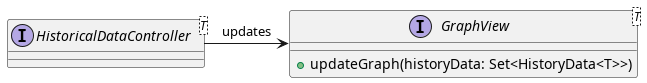
\includegraphics[width=\textwidth,height=\textheight,keepaspectratio]{magnani/uml/graph-view.png}
\caption{UML diagram of the graph view}
\label{magnani:uml:graph-view}
\end{figure}

\paragraph{Problem} How to handle the display of the new data.
\paragraph{Solution} I chose to refresh all the data each update for design simplicity.
Another way would have been to send only the new data from the graph controller to the view,
this would have required the view to decide whether to discard the oldest data record,
and due to time constraints, I just decided to go with the simplest way.
It also allowed me to better separate the logic and view, in fact it's the controller
deciding what to display.



\chapter{Development}
\section{Automated testing}
We used unit testing especially on the model to prevent regressions, and we tested observable behaviour only.
Our unit test suite uses JUnit.
We decided not to test UI components, since our UI is not the main focus,
and other areas of the model would benefit more from more granular testing. 

Tested classes:
\begin{itemize}
	\item Temperature
	\item DurationConverter
	\item Outlets
	\item temperaturechangers
	\item Logger
\end{itemize}

\subsection{Michele Ceccacci}
\begin{itemize}
	\item TemperatureTest
	\item AirqualityStateTest
	\item AbstractTemperatureChangerTest
	\item AirConditioningTest
	\item HeatingTest
	\item LoggerImplTest
\end{itemize}

\subsection{Simone Magnani}
\begin{itemize}
	\item BoundsTest
	\item LimitTest
	\item ClockImplTest
	\item SimpleActuatorTest
	\item AbstractActuatedDeviceTest
	\item SimpleLockTest
	\item TemperatureSchedulerTest
	\item MechanizedWindowTest
\end{itemize}


\section{Workflow}
The first step in our process was domain analysis, and then the insights gained were applied by modeling 
the project's main interfaces by using UML.
We used Git as our DCVS. We used gitflow and feature branching, with dev as our development branch,
and main as our stable branch for releases. The workflow is based on pull requests and forks, allowing for asynchronous feedback when needed.
Group meeting were only needed to discuss refactors. 


\subsection{Michele Ceccacci}

\begin{itemize}
    \item Utility classes
    \begin{itemize}
        \item \texttt{homer.common.temperature.*} 
		\item \texttt{homer.common.time.DurationConverter}
    \end{itemize}
	\item Model
	\begin{itemize}
		\item \texttt{homer.model.temperaturechangers.*}
		\item \texttt{homer.model.airquality.*}
	\end{itemize}
	\item Logger
	\begin{itemize}
		\item \texttt{homer.view.logger.*}
	\end{itemize}
	\item JavaFx view
	\begin{itemize}
		\item \texttt{homer.view.javafx.deviceview.*}
		\item \texttt{homer.view.javafx.JFXDeviceViewer} Responsible for most of the implementation
		\item \texttt{homer.view.javafx.*} Did most of the work on JFXDeviceViewer and everything in the other classes.
	\end{itemize}

\end{itemize}

I contributed to the architecture of DeviceViewer and the Controller class.

I also have minor contributions to the controllerImpl class, namely sending updates on temperature and air quality changes.
Whenever i noticed repeated code in the codebase i took charge of implementing a common solution, such as DurationConverter.

\subsection{Simone Magnani}
\begin{itemize}
    \item Utility classes
    \begin{itemize}
        \item \texttt{homer.common.bounds.*} for the abstraction of boundary values
        \item \texttt{homer.common.history.*} for the concept of data associated to a time
        \item \texttt{homer.common.limit.*} for a common and reusable way to limit values
        \item \texttt{homer.common.time.Clock*} for the concept of tracking custom time
    \end{itemize}
    \item For the simulation core
    \begin{itemize}
        \item \texttt{homer.core.*}
        \item \texttt{homer.view.sim.*}
    \end{itemize}
    \item For the implementation of the temperature scheduler
    \begin{itemize}
        \item \texttt{homer.controller.scheduler.*}
        \item \texttt{homer.model.scheduler.*}
        \item \texttt{homer.view.scheduler.*}
    \end{itemize}
    \item For the implementation of the graphs
    \begin{itemize}
        \item \texttt{homer.controller.history.*}
        \item \texttt{homer.model.history.*}
        \item \texttt{homer.view.graph.*} 
    \end{itemize}
    \item Devices
    \begin{itemize}
        \item \texttt{homer.model.lock.*}
        \item \texttt{homer.model.thermometer.*}
        \item \texttt{homer.model.environment.*} for the concept of physical environment
        \item \texttt{homer.model.actuator.*} for the concept of actuator and the abstraction of actuated devices
        \item \texttt{homer.model.blinds.*}
        \item \texttt{homer.model.door.*}
        \item \texttt{homer.model.window.*}
    \end{itemize}
\end{itemize}

I have contributed to the establishing of the architecture eg. \texttt{Device} and \texttt{Controller} interfaces.

When I had some ideas that could be used by someone else eg. \texttt{Environment, Bounds, Limit},
I would open a pull request, which allowed everyone to be aware of it, and who could chime in and provide their feedback.

I have also contributed in minor parts to the entrypoint and \texttt{Controller} implementation, for the integration of my code,
and \texttt{JFXDeviceViewer}.


\section{Development Notes}

\subsection{Michele Ceccacci}
\begin{itemize}
	\item \textbf{Optional}s were used when the value could either be present or not
	\item \textbf{Streams} were used to access and modify data, especially data that used optional types
	\item \textbf{Records} to make data immutability more explicit, and to avoid reimplementing constructors/HashCode methods
	\item \textbf{Lambda} functions and functional interfaces were used to make code more readable and often complemented streams 
	\item \textbf{JavaFX} was used to develop the main view.
\end{itemize}
\subsection{Simone Magnani}

\begin{itemize}
    \item \textbf{Generics and bounded generics} used in several parts of my code
    \begin{itemize}
        \item \url{https://github.com/progetto-oop-22-23/OOP22-HOMER/blob/main/src/main/java/homer/common/limit/Limit.java#L23}
    \end{itemize}
    \item \textbf{Lambda expressions}
    \begin{itemize}
        \item \url{https://github.com/progetto-oop-22-23/OOP22-HOMER/blob/main/src/main/java/homer/controller/scheduler/TemperatureCommandsImpl.java#L12}
    \end{itemize}
    \item \textbf{Functional interfaces} such as \texttt{Function}, \texttt{Supplier}, \texttt{BiConsumer}
    \begin{itemize}
        \item \url{https://github.com/progetto-oop-22-23/OOP22-HOMER/blob/main/src/main/java/homer/controller/scheduler/TemperatureCommand.java#L45}
    \end{itemize}
    \item \textbf{Stream}
    \begin{itemize}
        \item \url{https://github.com/progetto-oop-22-23/OOP22-HOMER/blob/main/src/main/java/homer/model/scheduler/TimeSchedulerImpl.java#L57}
    \end{itemize}
    \item \textbf{Optional}
    \begin{itemize}
        \item \url{https://github.com/progetto-oop-22-23/OOP22-HOMER/blob/main/src/main/java/homer/controller/scheduler/TemperatureSchedulerController.java#L81}
    \end{itemize}
    \item \textbf{Record} for the implementation of \texttt{HistoryData}
    \begin{itemize}
        \item \url{https://github.com/progetto-oop-22-23/OOP22-HOMER/blob/main/src/main/java/homer/common/history/HistoryData.java#L12}
    \end{itemize}
    \item \textbf{JavaFX} for the implementation of the sim, scheduler and graph views
    \begin{itemize}
        \item \url{https://github.com/progetto-oop-22-23/OOP22-HOMER/blob/main/src/main/java/homer/view/sim/SimManagerViewFxImpl.java#L20}
    \end{itemize}
    \item \textbf{ControlsFX} for the range slider
    \begin{itemize}
        \item \url{https://github.com/progetto-oop-22-23/OOP22-HOMER/blob/main/src/main/java/homer/view/scheduler/AddTemperatureScheduleViewFx.java#L28}
    \end{itemize}
\end{itemize}

To allow the air quality graphs FlowPane (placed inside of a ScrollPane) to automatically resize these two lines were used \url{https://stackoverflow.com/a/36264110}.


\chapter{Final comments}

\section{Self evaluation and final comments}

\subsection{Michele Ceccacci}
This project definitely improved my teamworking and software architecture skills. 
This was my first time participating in a greenfield project this big, and my first time 
taking architectural decisions that would carry over the whole software's lifecycle. 
In my previous work experience and open source contributions, i was more focused on  adding new features 
to an existing product or bugfixing, rather than actual softare architecture.
I was already proficient at git, but i still made some occasional mistakes.
I think that working in a team without a more senior figure acting as lead definitely 
made me more self reliant, and allowed me to dig deeper into problems.

\subsection{Simone Magnani}

Although this was not my first project of such dimensions to be designed from
scratch, it was the first one to be made in a team, and the first one where I
had the awareness that certain design choices had a name and are commonly used.
Altough the minimum requirements were met, I expected to reach further.
I now feel to have grasped how git works and am comfortable in using it in collaborative projects.
I will definitely carry over the knowledge I have acquired in architecture design and design patterns
onto my future projects.


\appendix
\chapter{User guide}

The main view is divided in two sections horizontally. \newline
Above there are 3 tabs: DEVICES, SCHEDULER and GRAPHS. \newline
At the bottom there is the SIMULATION information and control section, which reports the simulation time and the time rate, and allows the user to pause and resume the simulation, or change the time rate. \newline
In the DEVICES tab, there is an add window button. After selecting a device,
it will be created (and will be inserted at the bottom). Each device has a remove device button
used to disconnect it, and may have some kind of utility to set its state. \newline
In the SCHEDULER tab, the user can select the desired temperature range in time of the day intervals (schedule). \newline
No interval can be overlapping with another. The application will prevent the user from trying to do so, and notify them. \newline
When a schedule is present, the domotic controller will try to attain the desired parameters, provided that:
\begin{itemize}
	\item A thermometer is connected
	\item For heating: a heater is connected
	\item For cooling: an air conditioner is connected
\end{itemize}
In the GRAPHS tab, the user can visualize temperature, global consumption, and air quality parameters, logged at intervals of 1 hour. \newline
In order to visualize temperature and air quality parameters, either a thermometer or an air quality sensor, respectively, should be connected.

%TODO: describe outlet view.

\chapter{Lab Assignments}

\section{simone.magnani7@studio.unibo.it}

\begin{itemize}
 \item Laboratorio 07: \url{https://virtuale.unibo.it/mod/forum/discuss.php?d=117044#p173103}
 \item Laboratorio 09: \url{https://virtuale.unibo.it/mod/forum/discuss.php?d=118995#p175305}
 \item Laboratorio 10: \url{https://virtuale.unibo.it/mod/forum/discuss.php?d=119938#p176561}
 \item Laboratorio 11: \url{https://virtuale.unibo.it/mod/forum/discuss.php?d=121130#p177406}
\end{itemize}


\bibliographystyle{alpha}
\bibliography{13-template}

\end{document}
